% This must be in the first 5 lines to tell arXiv to use pdfLaTeX, which is strongly recommended.
\pdfoutput=1
% In particular, the hyperref package requires pdfLaTeX in order to break URLs across lines.

\documentclass[11pt]{article}

% Change "review" to "final" to generate the final (sometimes called camera-ready) version.
% Change to "preprint" to generate a non-anonymous version with page numbers.
\usepackage[preprint]{acl}

\usepackage{times}
\usepackage{pgfplots}
\usepackage{latexsym}
\usepackage{amssymb}
\usepackage{amsmath}
\usepackage{pifont}
\usepackage[T1]{fontenc}
\usepackage[utf8]{inputenc}
\usepackage{microtype}
\usepackage{inconsolata}
\usepackage{graphicx}

\usepackage[inline]{enumitem}
\usepackage{booktabs}
\usepackage{makecell}
\usepackage{standalone}
\usepackage{caption}
\usepackage{xcolor}
\usepackage{xspace}
\usepackage{multirow}
% \usepackage{showframe}

\usepackage[most]{tcolorbox}
\usepackage{etoolbox}
\tcbuselibrary{breakable}


\pgfplotsset{compat=1.16}
\usepgfplotslibrary{statistics, groupplots}
\usepgflibrary{plotmarks}
\usetikzlibrary{calc, patterns, matrix, positioning, shapes, shadows, shapes.geometric, arrows.meta}

\definecolor{ibm1}{HTML}{0077BB}
\definecolor{ibm2}{HTML}{33BBEE}
\definecolor{ibm3}{HTML}{EE7733}
\definecolor{ibm4}{HTML}{EE3377}
\definecolor{ibm5}{HTML}{CC3311}

\definecolor{grad1}{HTML}{364B9A}
\definecolor{grad2}{HTML}{6EA6CD}
\definecolor{grad3}{HTML}{C2E4EF}
\definecolor{grad4}{HTML}{FEDA8B}
\definecolor{grad5}{HTML}{F67E4B}



\newcounter{prompt}
\newtcolorbox[use counter=prompt]{promptbox}[2][]%
   {
    enhanced jigsaw,
    breakable,
    boxrule=0mm,
    colback=white, colframe=gray!50!black,
    top=0mm,bottom=1mm,left=1mm,right=1mm,
    arc=1mm,
    title={\textbf{Prompt \thetcbcounter: #2}},
    borderline={0.5pt}{0pt}{gray!50!black, rounded corners},
    #1,
}
\AtBeginEnvironment{promptbox}{\small \sffamily}


% \title{\textsc{HintsOfTruth}: A Multimodal Dataset For Checkworthiness Detection}
\title{\textsc{HintsOfTruth}: A Multimodal Checkworthiness Detection Dataset with Real and Synthetic Claims}

% \title{\textsc{HintsOfTruth}: Checkworthiness Detection Dataset with Real and Synthetic Images and Claims}
% \title{\textsc{HintsOfTruth}: A Checkworthiness Detection Dataset Combining Real and Synthetic Visual Claims}
% \title{Winds of Truth: A Multimodal Human-Centered Misinformation Benchmark}
% \title{Tail Winds of Truth: A Human-Centered Misinformation Benchmark}


\newcommand{\university}{\includegraphics[height=1.4em]{images/key_emoji.png}}
\newcommand{\institute}{\includegraphics[height=1.4em]{images/moutain_emoji.png}}
\newcommand{\lugano}{\includegraphics[height=1.4em]{images/wave_emoji.png}}

\author{
 \textbf{Michiel van der Meer\textsuperscript{\institute,\university}},
 \textbf{Pavel Korshunov\textsuperscript{\institute}}, \\
 \textbf{S\'{e}bastien Marcel\textsuperscript{\institute}},
 \textbf{Lonneke van der Plas\textsuperscript{\institute, \lugano}}
\\
\\
 {\small \institute} Idiap Research Institute, Martigny, Switzerland,\\
 {\small \university} Leiden University, Leiden, The Netherlands,\\
 {\small \lugano} Università della Svizzera Italiana, Lugano, Switzerland
\\
\\
%    \texttt{e@ma.il}
}


% Checkmark and crossmark
\newcommand{\cmark}{\ding{51}}%
\newcommand{\xmark}{\ding{55}}%

\newcommand{\hiot}{\textsc{HintsOfTruth}\xspace}

\begin{document}
\maketitle
\begin{abstract}
Misinformation can be countered with fact-checking, but the process is costly and slow. Identifying checkworthy claims is the first step, where automation can help scale fact-checkers' efforts. However, detection methods struggle with content that is
\begin{enumerate*}[label=(\arabic*)]
    \item multimodal,
    \item from diverse domains, and
    \item synthetic
\end{enumerate*}.
We introduce \hiot, a public dataset for multimodal checkworthiness detection with $27$K real-world and synthetic image/claim pairs. The mix of real and synthetic data makes this dataset unique and ideal for benchmarking detection methods.
We compare fine-tuned and prompted Large Language Models (LLMs). We find that well-configured lightweight text-based encoders perform comparably to multimodal models but the first only focus on identifying non-claim-like content. Multimodal LLMs can be more accurate but come at a significant computational cost, making them impractical for large-scale applications. When faced with synthetic data, multimodal models perform more robustly. \\
\includegraphics[width=.9em]{images/github.png} \url{https://hintsoftruth.github.io/}
\end{abstract}


\section{Introduction}
\label{sec:intro}
Online misinformation spreads rapidly via social networks and deceptive websites posing as legitimate news sources \citep{del2016spreading, rocha2021impact, Ecker2024}. This influences voting behavior \citep{ribeiro2017everything} and pollutes the digital information space \citep{greenspan2021pandemics, sharma2019combating}. Misinformation tactics include decontextualization (e.g., wrongly presenting image-based evidence) and providing incomplete information \citep{kreps2022all}. Generative AI, like ChatGPT \citep{openai2023chatgpt} for text and Midjourney \citep{midjourney2023midjourney} for images, has worsened the issue by enabling large-scale alteration or fabrication of news narratives \citep{zhou2023synthetic, chen2024combating}. Given these developments, continuous verification of multimodal information is a key challenge \citep{abdelnabi2022open, singh2022predicting}.

\begin{figure}[t]
    \centering
    \begin{tikzpicture}
        % Checkworthy
        % 'photograph shows a tsunami 1/2 second before it struck the island of sumatra.'
        \node[] at (0,0) {\includegraphics[width=4cm]{images/figure_1_checkw.png}};
        \node[draw=black, align=center, text width=3cm] at (4,0) {photograph shows a tsunami 1/2 second before it struck the island of Sumatra.};
        \node[] at (2, 1.5) {\textbf{Checkworthy \cmark}};

        % Non checkworthy
        % 'A man in a black hat and blue shirt taking a picture on the side of an urban street.'
        \node[] at (0,-3.4) {\includegraphics[width=4cm]{images/figure_1_non_checkw.png}};
        \node[draw=black, align=center, text width=3cm] at (4,-3.4) {a man in a black hat and blue shirt taking a picture on the side of an urban street.};
        \node[] at (2, -1.8) {\textbf{Non-checkworthy \xmark}};
    \end{tikzpicture}
    \caption{Examples of the multimodal checkworthiness detection task.}
    \label{fig:example-first-page}
\end{figure}

Media gatekeepers, including news publishers and fact-checking services, verify content veracity, but manual fact-checking is costly and time-consuming \citep{nakov2021automated}. Therefore, selecting which claims to fact-check is a major challenge, as misinformation far exceeds verification capacity. Automated approaches can help by identifying \textbf{checkworthy} claims \citep{nakov2018overview, konstantinovskiy2021toward}, see Figure~\ref{fig:example-first-page} for an example, or in other stages in the fact-checking pipeline (Figure~\ref{fig:fact-checking-pipeline}).


However, existing automated checkworthiness detection methods \begin{enumerate*}[label=(\arabic*)]
    \item have poor support for multimodal content,
    \item have only been tested in a handful of domains,
    \item have unknown capabilities on synthetic media, and
    \item do not consider compute cost as a factor.
\end{enumerate*} \citep{akhtar-etal-2023-multimodal}.
First, modern misinformation often includes mixed forms of media, such as images or videos \citep{dufour2024ammeba}, yet it is unclear if detection methods effectively integrate visual data \citep{alam2023overview}.
Second, strategies for misinformation detection vary by domain \citep{ecker2022psychological, chen2021persuasion, lasser2023alternative}, raising concerns about generalizability, especially, for practical applications \citep{jiang2018linguistic, monteith2024artificial}.
Third, ubiquitous access to generative models is reshaping misinformation \citep{xu2023combating}, warranting the evaluation of detection methods on synthetic content.
Lastly, while Large Language Models (LLMs) perform well, their high compute cost may render large-scale checkworthiness detection impractical \citep{augenstein2024factuality}, though the exact tradeoffs are unknown.

This paper introduces \hiot, the first publicly available multimodal dataset of image-text pairs containing both real-world and synthetically generated checkworthy and non-checkworthy claims. We source real claims from datasets like 5Pils \citep{tonglet2024image}, Multiclaim \citep{pikuliak2023multilingual}, Flickr30K \citep{hodosh2013framing}, and SentiCap \citep{sharma2018conceptual}. Synthetic images and text are generated using Flux \citep{flux2024}, StableDiffusion 3.5 \citep[][SD]{stablediff}, Llava \citep{li2024llavanext}, and BLIP \citep{li2022blip}. We evaluate recent text and image models, from lightweight ones like TinyBERT \citep{tinybert} for scalability to large, multimodal models like Pixtral \citep{mistral2024pixtral}. These evaluations reveal model limitations and guide practical decisions in checkworthiness detection.

\paragraph{Contributions}
We present: \begin{enumerate*}[label=(\arabic*)]
    \item \hiot, a novel dataset for multimodal checkworthiness detection from diverse sources, with an established connection between images and textual claims, that can be used as a benchmark for checkworthiness detection models,
    \item synthetic counterparts of images and claims in the dataset, which has not been explored in the context of checkworthiness, and
    \item an extensive set of experiments demonstrating the limits of state-of-the-art detection methods.
\end{enumerate*}

% == Approach before 2024-09-30 ==
% \begin{description}
%     \item[RQ1] In what ways do fact-checkers need to be supported in fact-checking?
%     % Approach:
%     %   [x] 1) Look at fact-checking pipeline and see what has been identified so far
%     %   [x] 2) See if we can identify tasks which we the AI can do to help
%     %   3) Verify with specific fact-checkers to see if they like using AI in these tasks
%     \item[RQ2] How to realistically augment existing datasets with generative models like (M)LLMs?
%     % Approach:
%     %   1) Look at existing datasets and see if they cover the tasks in RQ1
%     %   2) See if they are diverse: languages, modalities, contexts.
%     %   3) See if we can generate synthetic data that covers the missing parts
%     \item[RQ3] Does synthetically generated misinformation improve hybrid (human--AI) fact-checking?
%     % Approach:
%     %   1) Benchmark standard approaches for the tasks on the existing datasets
%     %   2) Benchmark the same approaches on the enhanced datasets
%     %   [3) Maybe show that humans also struggle with the enhancements]
% \end{description}
% == ==


% Reiterate problem of long-tailed ness? famous entities are recognized correctly by pretrained models, but unfamiliar ones are not.



% Specific idea: group existing claims together to find those with similar narratives
% Create a model for generating claims given a narrative
% Bundle new claims together in a benchmark dataset that can adapt to new narratives

% How many fact-checking articles show that the misinformation is the result of _manipulation_ vs. _fabrication_?
% Text - true, fake, edited
% Image - true, fake, manipulated
% Combination - matching, mismatching
% enhance with metadata on TIME, LOCATION, SPEAKER


\section{Related Work}
\subsection{Human-Centered Fact-Checking}
Recent research on human-centered AI has emphasized developing tools that augment humans \citep{akata2020research, nakov2021automated}. In the field of fact-checking, such tools would complement human fact-checkers in their work \citep{micallef2022true, graves2017anatomy}, allowing experts to control \emph{what} and \emph{how} to fact-check \citep{das2023state}.
% In this framework, technology primarily assists in filtering irrelevant information, while humans retain responsibility for drawing nuanced conclusions. By breaking down the fact-checking process into manageable components, this approach creates a more interactive workflow, aiding in evidence discovery and articulating reasoning behind fact-checks. This collaborative model enhances both the efficiency and transparency of the fact-checking process, leveraging the strengths of both human expertise and technological support.
% Research has shifted from focusing on end-to-end automated fact-checking to ensuring that we develop technology that augments humans instead of replacing them \citep{akata2020research,nakov2021automated}.
% Existing practitioners want support tools that can be integrated into existing workflows. Further, NLP tools are not accurate enough for complete end-to-end fact-checking. Hence, human-centered fact-checking is best served by creating approaches that work hand in hand with fact-checkers \citep{das2023state}.
% This means letting the human expert decide \emph{what} and \emph{how} to fact-check. Support should come from wading out lots of clearly irrelevant information, coming to the right conclusions is best done by the human.
% We can break down the task into smaller components to make it more interactive. Humans can be helped to find evidence and connect the reasoning behind fact-checks.

\begin{figure}
    \centering
\resizebox{\columnwidth}{!}{%
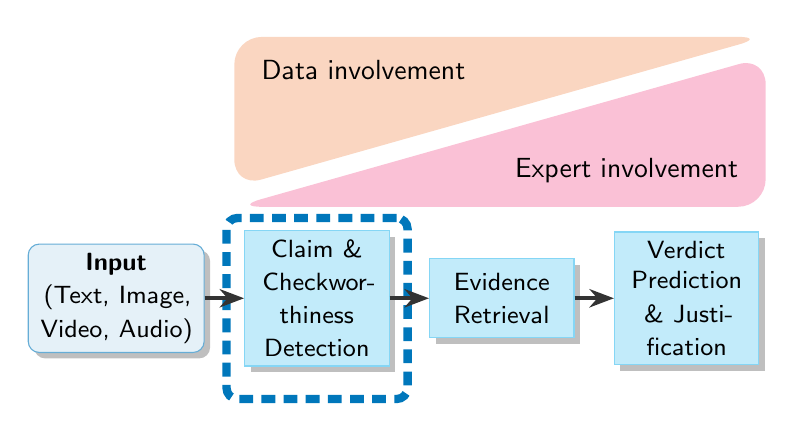
\begin{tikzpicture}[node distance=1cm and 0.5cm, auto]
    \tikzstyle{startstop} = [
        rectangle,
        rounded corners,
        text width=2cm,
        minimum height=1cm,
        text centered,
        draw=ibm1!60,
        fill=ibm1!10,
        font=\sffamily,
        drop shadow
    ]
    \tikzstyle{expert-inv} = [
        rectangle,
        minimum width=5cm,
        minimum height=1cm,
        draw=ibm5!60,
        fill=ibm5!30,
    ]
    \tikzstyle{process} = [
        rectangle,
        text width=1.6cm,
        minimum height=1cm,
        text centered,
        draw=ibm2!60,
        fill=ibm2!30,
        font=\sffamily,
        drop shadow
    ]
    \tikzstyle{text-only} = [
        font=\sffamily,
    ]
    \tikzstyle{highlight} = [
        rectangle,
        minimum width=2.3cm,
        minimum height=2.3cm,
        draw=ibm1,
        rounded corners,
        line width=3pt,
        fill=none,
    ]

    \tikzstyle{arrow} = [line width=1.3pt, ->, >=Stealth, draw=black!80]

    \node (input) [startstop] {\small \textbf{Input}\\  (Text, Image, Video, Audio)};
    \node (stage1) [process, right=of input] {\small Claim \& Checkworthiness Detection};
    \node (stage2) [process, right=of stage1] {\small Evidence Retrieval};
    \node (stage3) [process, right=of stage2] {\small Verdict Prediction\\ \& Justification};
    \node (highlight) [highlight, dashed, dash pattern=on 5pt off 3pt, below right=0cm and 0cm of stage1.base, xshift=-1.2cm, yshift=.55cm] {};

    \draw [arrow] (input) -- (stage1);
    \draw [arrow] (stage1) -- (stage2);
    \draw [arrow] (stage2) -- (stage3);

    \node (data-top-left) [above=2.5cm of input, xshift=1.5cm] {};
    \node (data-top-right) [right=6.5cm of data-top-left] {};
    \node (data-bottom-left) [below=1.66cm of data-top-left] {};
    \fill[ibm3, rounded corners=10pt, opacity=0.3]
        (data-top-left.center) --
        (data-top-right.center) --
        (data-bottom-left.center) --
        cycle;
    \node (exp-bottom-left) [below=.001cm of data-bottom-left] {};
    \node (exp-top-right) [below=.001cm of data-top-right] {};
    \node (exp-bottom-right) [below=1.66cm of exp-top-right] {};
    \fill[ibm4, rounded corners=10pt, opacity=0.3]
        (exp-bottom-left.center) --
        (exp-top-right.center) --
        (exp-bottom-right.center) --
        cycle;
    \node [text-only, below right=.05cm and .1cm of data-top-left] {Data involvement};
    \node [text-only, above left=.05cm and .1cm of exp-bottom-right] {Expert involvement};
\end{tikzpicture}%
}
    \caption{The fact-checking pipeline from \citet{akhtar-etal-2023-multimodal}, visualized the amount of data and expert effort required. We focus on the highlighted stage. }
    \label{fig:fact-checking-pipeline}
\end{figure}

Crucially, as shown in Figure~\ref{fig:fact-checking-pipeline}, the fact-checking pipeline involves handling large amounts of data by experts. Especially in the early stages of the pipeline, experts can only spend a small amount of time per claim in assessing whether it is \textbf{checkworthy}. Natural Language Processing (NLP) technology enables various types of support, especially when dealing with scale \citep{vandermeer2024facilitating, procter2023some}, to simplify the problem \citep{chen2022generating, bonet2024run}, or to combat cognitive biases \citep{soprano2024cognitive}. These diverse applications demonstrate the potential of NLP in supporting the fact-checking process.

% For instance, in the fact-checking pipeline \citep{liu2023human}. For instance, it can help counteract the cognitive biases that human fact-checkers often face \citep{soprano2024cognitive}, or
% Generating claims from abstract narratives helps in testing this repurposing
% Additionally, NLP-generated explanations have been shown to enhance the accuracy of lay users while simultaneously improving the perceived usefulness, understandability, and trust in AI systems \citep{schmitt2024role}.
% Other applications include the identification of relevant experts \citep{zhang2023newsquote}, question decomposition to simplify complex claims \citep{chen2022generating}, and the implementation of the 5W1H (Who, What, When, Where, Why, and How) approach for comprehensive claim investigation \citep{bonet2024run, tonglet2024image}.

\subsection{Misinformation in the Age of LLMs}
LLMs play a significant role in both detecting and generating misinformation. Recent work integrates LLMs into fact-checking frameworks \citep{geng2024multimodal}, although methods are shown to generalize poorly across time \citep{stepanova-ross-2023-temporal}. Nonetheless, LLMs look promising when applied to text-based checkworthiness detection \citep{majer2024claim}. Reviews of LLM-generated multimedia highlight the open challenges \citep{lin2024detecting, augenstein2024factuality}. For instance, large amounts of synthetic misinformation have the potential to impact the quality of future LLMs \citep{pan2023risk}, and misinformation generated by GPT-4 may be harder to detect than that written by humans \citep{chen2024combating}.

\subsection{Multimodal Resources}
Existing work on fact-checking emphasizes empirical research, which involves extensively benchmarking fact-checking methods \citep{schlichtkrull2024averitec, papadopoulos2024verite}, often using distant supervision \citep{nakamura2020fakeddit, zlatkova2019fact}. Most multimodal datasets investigate the out-of-context use of images and claims \citep{luo2021newsclippings, tonglet2024image}, or whether claims are reflected in an image between claim and image \citep{yoon2024assessing, papadopoulos2023synthetic}. Few datasets exist that
\begin{enumerate*}[label=(\arabic*)]
    \item check whether the image contributes new information \citep{liu2024mmfakebench}, or
    \item contain synthetically generated data \citep{xu2023combating, seow2022comprehensive}
\end{enumerate*}. The few efforts on multimodal checkworthiness indicate that textual data, whether through OCR or by focusing on claims only, is sufficient for state-of-the-art performance \citep{frick2023fraunhofer}. More extensive experiments on varied types of data with complex image use, across domains, are needed to further examine this finding.
% While performance metrics, such as classification accuracies are important signals of a system's capabilities, these metrics report only general trends, and do not reveal further details about \emph{what type}, or \emph{why} something was classified as misinformation. Unfortunately, few resources that provide such a human-centered perspective are available:
% Human-centered fact-checking datasets
% \begin{enumerate*}[label=(\arabic*)]
%     \item Some datasets, like AVeriTeC \citep{schlichtkrull2024averitec} and ClaimDecomp \citep{chen2022generating}, include question and answers (Q\&A), such that a system may learn to decompose claims into relevant subquestions.
% \end{enumerate*}


\section{Method}
\label{sec:method}
We introduce the multimodal checkworthiness task definition, how we obtain the real-world data underlying \hiot, and how we generate synthetic samples to augment our dataset.

\subsection{Task Definition: Multimodal Checkworthiness Detection}
\label{sec:task-definition}
Given a textual claim $c$ and an image published alongside the claim $i$, predict whether the pair is worthy of fact-checking $p(i,c) = 1$. In checkworthiness detection, the following questions are answered:
\begin{enumerate*}[label=(\textbf{Q\arabic*})]
    \item Does the text contain a verifiable factual claim?
    \item Is the claim potentially harmful, urgent, and up-to-date?
\end{enumerate*}
The task definition is derived from \citet{barron2020overview}, which also formed the basis for the canonical dataset for multimodal checkworthiness detection, CheckThat! 2023 Task 1A \citep{alam2023overview}.

To establish that an image provides meaningful context to a claim and is necessary for assessing the pair's checkworthiness, we also consider the following contextualized questions:
\begin{enumerate*}[label=(\textbf{Q\arabic*})]
    \setcounter{enumi}{2}
    \item Is the content of the claim reflected in the image?
    \item Does the image contribute extra information to the claim?
\end{enumerate*}
These two questions help identify \emph{complex} image use, which will test the multimodal capabilities of checkworthiness detectors \citep{dufour2024ammeba}.

\subsection{Getting Checkworthy Image/Claim Pairs}
We set out to obtain image/claims pairs that we can deem checkworthy. We rely on data stemming from fact-checking articles, as claims in these articles have already been checked. Fact-checking articles are written by experienced fact-checkers and contain rich contextual information. In practice, claims are often sourced from social media platforms. We obtain our data from two sources:
\begin{description}[itemsep=-5pt, leftmargin=0pt, topsep=0pt, partopsep=0pt]
    \item[5Pils] \citep{tonglet2024image}. 5Pils contains extracted images, claims, and contextual questions about claims from news sources in India, Kenya, and South Sudan. Through the use of contextual questions, images in this dataset are ensured to have a relationship with the claim.
    \item[Multiclaim] \citep{pikuliak2023multilingual} contains URLs to a wide array of fact-checking articles and their respective claims but needs to be scraped and filtered for images. We retain those claims for which \begin{enumerate*}[label=(\arabic*)]
    \item we find images in close proximity, and
    \item explicitly refer to visual information
    \end{enumerate*}. See Appendix~\ref{app:multiclaim-extraction} for additional details.
\end{description}

\subsection{Non-checkworthy Image/Claim Pairs}
We also need image/text pairs that are not checkworthy. We resort to strategies derived from the task definition for obtaining negative instances. We select samples from datasets that we consider not checkworthy because they answer `no' to any of the guiding questions posed in Section~\ref{sec:task-definition}. The strategies select:
\begin{description}[itemsep=-5pt, leftmargin=0pt, topsep=0pt, partopsep=0pt]
    \item[Non-factual (Q1)] claims, such as subjective opinions or facts that cannot be verified using external information. The dataset representing this strategy is \textbf{SentiCap} \citep{sharma2018conceptual}.
    \item[Non-relevant (Q2)] statements that are not harmful, not about breaking news, not up-to-date, or not relevant to news topics. The dataset representing this strategy is \textbf{Flickr30K} \citep{hodosh2013framing}, though there are many other resources containing arbitrary image-text pairs (see Appendix~\ref{app:image-captions}).
    \item[No cross-modal connection (Q3)] images we know have a deep connection with a text but with the image swapped to no longer make sense. The dataset representing this strategy is \textbf{Fakeddit} \citep{nakamura2020fakeddit}.
\end{description}
To incorporate the fourth guiding question (\textbf{Q4}), we filter out claims from any of the stated datasets that do not explicitly refer to multimodal content. This way, we encourage that the samples with basic image use (i.e., those pairs where the claim does not refer to the image) are excluded from our dataset. We combine the checkworthy and non-checkworthy samples into \hiot, our novel multimodal checkworthiness dataset that spans multiple domains.

\begin{table*}[ht]
  \centering
  \resizebox{\textwidth}{!}{%
  \begin{tabular}{@{}l l c r p{7.7cm}@{}}
    \toprule
    \textbf{Dataset} & \textbf{Source / Subset} & \textbf{Checkworthy} & \textbf{Size} & \textbf{Description} \\
    \midrule
    CheckThat 2023 Task 1A
      & Twitter
      & Mixed
      & 3,175
      & Tweets on COVID-19, technology, climate change. \\[1mm]
    \midrule
      & 5Pils
      & \cmark
      & 1,676
      & News articles from India, Kenya, and South Sudan. \\[0.5mm]
      & Multiclaim
      & \cmark
      & 3,048
      & Social media posts in a general domain. \\[0.5mm]
      & SentiCap
      & \xmark
      & 3,171
      & Captions with sentiment injection. \\[0.5mm]
      & Flickr30K
      & \xmark
      & 30,000
      & Image captions from a general domain. \\[0.5mm]
      & Fakeddit
      & \xmark
      & 1,382
      & Reddit posts from a general domain. \\[1mm]
      \cmidrule{2-5}
      \hiot & Mixed & Mixed & 12,277 & Mixed domain benchmark\\
    \midrule
    \multirow{2}{*}{\(\hiot\text{-aug}\)}
      & \textbf{5Pils}
      & Mixed
      & 1,676
      & Generated claims using BLIP, Llava. Generated images using Flux, StableDiffusion 3.5. \\[0.5mm]
      % & \textbf{5Pils} -- Text (LL)
      % & \cmark
      % & 1,676
      % & Generated text using Llava. \\[0.5mm]
      % & \textbf{5Pils} -- Img (F)
      % & \cmark
      % & 1,676
      % & Generated images using Flux. \\[0.5mm]
      % & \textbf{5Pils} -- Img (SD)
      % & \cmark
      % & 1,676
      % & Generated images using StableDiffusion 3.5. \\[0.5mm]
      & \textbf{Flickr30K}
      & \xmark
      & 30,000
      & Generated captions using BLIP, Llava. Generated images using Flux, StableDiffusion 3.5. \\
      % & \textbf{Flickr30K} -- Text (LL)
      % & \xmark
      % & 30,000
      % & Generated text using Llava. \\[0.5mm]
      % & \textbf{Flickr30K} -- Img (F)
      % & \xmark
      % & 30,000
      % & Generated images using Flux. \\[0.5mm]
      % & \textbf{Flickr30K} -- Img (SD)
      % & \xmark
      % & 30,000
      % & Generated images using StableDiffusion 3.5. \\
    \bottomrule
  \end{tabular}%
  }
  \caption{Overview of the datasets used in this study for multimodal checkworthiness. \(\hiot\) aggregates samples from five sources, and \(\hiot\text{-aug}\) contains synthetically generated variants.}
  \label{tab:datasets}
\end{table*}

\subsection{Generating Synthetic Samples}
\label{sec:method-generating}
Given the risks of synthetic misinformation \citep{dufour2024ammeba, papadopoulos2023synthetic, zhou2023synthetic}, we augment our dataset with additional claims and images generated using various publicly accessible models. Specifically, we employ two image generators to create images from claims and two multimodal models to generate claims from images. Our approach follows a simple cross-modality generation: models freely generate corresponding text or images without adversarial prompts \citep{perez2022ignore}. This allows us to examine how checkworthiness detection models respond to synthetic data. Labels are adjusted accordingly: synthetic \textbf{claims} are deemed \emph{non-checkworthy}, as models primarily generate non-relevant captions (see \textbf{Q2} in Section~\ref{sec:task-definition}), while synthetic \textbf{images} retain their original label, ensuring consistency with the claim’s content. \emph{Checkworthy} claims remain unchanged.




% ======== OTHER IDEAS ========
% Use SMISTS for evaluation or development? \citep{ma-etal-2024-simulated}

% One way to become human-centered is to take into account human and machine uncertainty with the aim of creating explainable processes. Another would be to let users override the system's predictions.

% What is the source of most misinformation? Some images that are contained in the claimreviews are pictures of videos.

% Look at big pre-training datasets and see if we can find a number of articles that are fake or in the mean time have been identified as misinformation.

% Basic versus Complex image use
% Data analysis for the CheckThat dataset, plus the new datasets that we end up using. We will let humans answer the four questions on a subset of the data we have in our dataset, and provide a final checkworthiness answer.
% Alternatively, can the strongest model classify the text with and without the image?

% Attribution methods
% Can we show, based on what samples are influential for making certain (mis)classifications, that the text is more important than the image?

% =============================



\section{Experiments}

\subsection{Data}
See Table~\ref{tab:datasets} for the datasets used in this paper. We use the canonical CheckThat! 2023 Task 1A dataset \citep[`CheckThat' henceforth,][]{alam2023overview} as training dataset and reference benchmark using its predefined train/test split, which represents the in-distribution scenario (models are trained and tested on the same dataset). CheckThat has a label ratio of .66/.34 between non-checkworthy and checkworthy samples. We use the test set of our dataset, \hiot (label ratio of .62/.38) for testing the detection methods fine-tuned on CheckThat, representing the cross-distribution scenario, which should be more challenging than in-distribution. We will make our dataset publicly available upon publication.



\subsection{Multimodal Checkworthiness Methods}
\label{sec:experimental-approaches}
We experiment with various state-of-the-art text-based, image-based, and multimodal encoders for checkworthiness detection, see Table~\ref{tab:models}. We use different model sizes to investigate the tradeoff between compute cost and task performance. We include single-modality models to identify whether both modalities are needed (i.e., checkworthiness can be assessed without leveraging cross-modal information). In addition, we distinguish between encoder-only and decoder-only models, to determine the difference between fine-tuning models on multimodal checkworthiness and In-Context Learning \citep[][]{dong2022survey}. Below, we describe the experimental setup for each type of approach. Additional information is available in Appendix~\ref{app:experimental-details}.
\begin{table}[t]
    \small
    \centering
    \begin{tabular}{@{}lllc@{}}
        \toprule
        \textbf{Model} & \textbf{Modality} & \textbf{Size} & \textbf{App.} \\
        \midrule
        TinyBERT & text & 14M & FT\\
        BERT-base & text & 109M & FT\\
        BERT-large & text & 335M & FT\\
        \midrule
        ResNet-26 & image & 16M & FT \\
        ViT-base & image & 86M & FT\\
        ViT-large & image & 303M & FT\\
        \midrule
        BLIP & text, image & 385M & FT\\
        BLIP2 & text, image & 1.17B & FT\\
        \midrule
        Llava  & text, image & 7.57B & ICL\\
        Pixtral & text, image & 12.4B & ICL\\
        \bottomrule
    \end{tabular}
    \caption{Models used for checkworthiness detection. Depending on the model, we fine-tune them (FT) or perform In-Context Learning (ICL).}
    \label{tab:models}
\end{table}

\paragraph{Fine-Tuning (FT)}
To fine-tune models for multimodal checkworthiness detection, we update all model parameters $\theta$ when predicting $p_{\theta}(i,c)$. We instantiate the models using pretrained versions, adding a single linear classification layer with a two-node output over their embeddings.\footnote{Single-logit was less stable and yielded inferior performance, see App. \ref{app:single-logit}.} We fine-tune our models with data from CheckThat using its predefined train/val/test split. Additionally, we tune a threshold parameter on the positive class probability, similar to a single-neuron sigmoid output \citep{ZOU20162, Korshunov_ICB_2019}. At various thresholds, we compute the True Positive Rate (TPR) and False Positive Rate (FPR), and we select the threshold for an FPR of $0.3$, prioritizing recall over precision (see App.~\ref{app:tuning-threshold}).

\paragraph{In-Context Learning (ICL)}
We evaluate the impact of $n$-shot learning (with $n=\{0,1,2,5\}$) and prompt verbosity. The verbose prompt instructions include guiding questions \textbf{Q1} through \textbf{Q4} (see Section~\ref{sec:task-definition}), while the succinct prompt only asks for an overall checkworthiness label. We experiment with two models:
\begin{enumerate*}[label=(\arabic*)]
    \item \textbf{Llava} \citep{liu2024visual}, using a Mistral-7B backend with a 32K token context.
    \item \textbf{Pixtral} \citep{mistral2024pixtral}, with a context size of 1024K.
\end{enumerate*}
Both models are chosen for their compatibility with standard hardware (up to a single H100 with 80GB VRAM) and accessibility, excluding non-local proprietary LLMs. Our experiments focus on zero-shot ICL with concise instructions to minimize token usage, though multiple setups are explored in Section~\ref{sec:cross-modal}.


\subsection{Research Questions}
Based on the criteria discussed in Section~\ref{sec:intro}, we conduct four experiments to address:
\begin{enumerate*}[label=(Q\arabic*)]
\item Does combining modalities influence checkworthiness detection performance?
\item How well do models generalize across domains?
\item How do models fare on synthetic data?
\item What is the tradeoff between compute cost and task performance?
\end{enumerate*}

\section{Results}
Table~\ref{tab:checkthat20231a} shows the in-distribution experiments results on CheckThat, and Table~\ref{tab:cross-dataset-perf} demonstrates the results on the non-synthetic, real part of \hiot, illustrating the cross-distribution experiments. We answer each research question individually step by step.


\begin{table}
    \centering
    \resizebox{.88\columnwidth}{!}{%
    \begin{tabular}{@{}lcccc@{}}
        \toprule
        \textbf{Model} & \textbf{Prec.} & \textbf{Rec.} & \textbf{F1} & \textbf{Acc.}\\
        \midrule
        TinyBERT         & 0.698 & 0.721 & 0.702 & 0.724\\
        BERT-base        & \underline{0.735} & 0.769 & 0.735 & 0.748\\
        BERT-large       & 0.726 & 0.760 & 0.723 & 0.735\\
        ResNet           & 0.595 & 0.600 & 0.596 & 0.641\\
        ViT-base         & 0.639 & 0.655 & 0.640 & 0.666\\
        ViT-large        & 0.654 & 0.670 & 0.658 & 0.686\\
        BLIP             &\textbf{0.782} & \underline{0.819} & \textbf{0.788} & \textbf{0.801}\\
        BLIP2            & \textbf{0.782} & \textbf{0.822} & \underline{0.786} & \underline{0.797}\\
        Llava (0-shot)   & 0.565 & 0.574 & 0.554 & 0.572\\
        Pixtral (0-shot) & 0.673 & 0.675 & 0.588 & 0.588\\
        \bottomrule
    \end{tabular}
    }
    \caption{(Macro-averaged) performance for the CheckThat! 2023 Task 1A benchmark.}
    \label{tab:checkthat20231a}
\end{table}


\begin{table*}
    \small
    \centering
    \begin{tabular}{@{}lccccccccc@{}}
        \toprule
        & 5Pils & \small Multiclaim & \small Flickr30K & \small SentiCap & \small Fakeddit& \multicolumn{4}{c}{Overall}\\
        \textbf{Model} & \textbf{Acc.} & \textbf{Acc.} & \textbf{Acc.} & \textbf{Acc.} & \textbf{Acc.} & \textbf{P.} & \textbf{R.} & \textbf{F1} & \textbf{Acc.}\\
        \midrule
        TinyBERT         & \underline{0.895} & \underline{0.871} & 0.787 & 0.734 & 0.493 & \underline{0.780} & \underline{0.795} & \underline{0.773} & \underline{0.775}\\
        BERT-base        & 0.702 & 0.638 & 0.582 & 0.799 & 0.805 & 0.682 & 0.688 & 0.684 & 0.694\\
        BERT-large       & 0.702 & 0.583 & 0.472 & \underline{0.807} & \textbf{0.836} & 0.648 & 0.653 & 0.649 & 0.659\\
        ResNet           & 0.491 & 0.388 & 0.713 & 0.671 & 0.681 & 0.560 & 0.557 & 0.558 & 0.587\\
        ViT-base         & 0.317 & 0.325 & 0.708 & 0.669 & 0.775 & 0.515 & 0.513 & 0.510 & 0.557\\
        ViT-large        & 0.416 & 0.333 & 0.703 & 0.642 & 0.780 & 0.530 & 0.528 & 0.527 & 0.565\\
        BLIP             & 0.770 & 0.551 & \underline{0.913} & 0.561 & 0.436 & 0.648 & 0.654 & 0.649 & 0.659\\
        BLIP2            & 0.892 & 0.803 & 0.739 & 0.697 & 0.648 & 0.756 & 0.770 & 0.752 & 0.755\\
        Llava (0-shot)   & 0.223 & 0.220 & 0.047 & 0.444 & \underline{0.833} & 0.319 & 0.310 & 0.312 & 0.326\\
        Pixtral (0-shot) & \textbf{0.942} & \textbf{0.934} & \textbf{0.923} & \textbf{0.939} & 0.627 & \textbf{0.891} & \textbf{0.907} & \textbf{0.896} & \textbf{0.899}\\
        \bottomrule
    \end{tabular}
    \caption{Test set of \hiot, performance per subset. The last four columns show the overall macro-averaged scores. Best scores per sub-dataset are shown in \textbf{bold}, with the second-best \underline{underlined}.}
    \label{tab:cross-dataset-perf}
\end{table*}

\subsection{Cross-modality Performance}
\label{sec:cross-modal}
% On CheckThat
On the CheckThat dataset, the strongest models are multimodal BLIP and BLIP2, which form the upper bound (see Table~\ref{tab:checkthat20231a}). Interestingly, the accuracies of text-only encoders are close to those of BLIP and BLIP2 (up to $93$\% of accuracy), suggesting that little visual information is required for accurate checkworthiness detection, in line with results found in \citet{frick2023fraunhofer}. Image-only encoders also achieve only $14$\% lower accuracy than the upper bound. The narrow gap between single and multimodal models shows the dataset's limited suitability for assessing multimodal capabilities. ICL-based methods perform surprisingly poorly, with considerable false positive rates of $30$\% and $39$\% for Llava and Pixtral.

% On HoT
For real data of \hiot, Pixtral forms the upper performance bound (see Table~\ref{tab:cross-dataset-perf}). The gap between text-only models and the upper bound is larger than in CheckThat ($-14$\% vs.\ $-7$\%). Surprisingly, TinyBERT outperforms larger text-only models and is second to only Pixtral. This suggests that a small model with a well-tuned classification threshold can be effective, which poses an interesting venue for smaller organizations with limited compute capacity. Image-only encoders perform worse ($-35$\% vs.\ upper bound) than others. Among multimodal models, BLIP2 excels, followed by Llava, aligning performance with parameter count (i.e., the bigger the model, the better its performance).

% Overall ICL
We investigate the impact of $n$-shot learning on LLava and Pixtral by varying the prompting setup for these ICL models in Figure~\ref{fig:icl-results-fewshot}. Performance on \hiot reveals that Pixtral and Llava have contrary behavior with an increase in context:
\begin{enumerate*}[label=(\arabic*)]
    \item Adding more examples with few-shot learning aids Llava but hurts the Pixtral model, and
    \item Llava can benefit from a long prompt in zero-shot cases, but Pixtral generally benefits from short prompts.
\end{enumerate*} This is a surprising finding as additional examples should inform a model better. Like before, we observe an oversensitivity to predicting a \emph{checkworthy} label. The wide context of Pixtral may have it confuse which image/claim pair is currently under scrutiny.
While CheckThat shows this behavior partially, \hiot provides a clearer pattern, attesting to the usefulness of our dataset.

\begin{figure}[t]
    \centering
    \includestandalone[width=\columnwidth]{plots/icl_performance}
    \caption{Few-shot performance with ICL on CheckThat (left) and \hiot (right).}
    \label{fig:icl-results-fewshot}
\end{figure}

\subsection{Domain Generalization}
Evaluating performance on each of the \hiot subsets shows (see Table~\ref{tab:checkthat20231a}) that while fine-tuned (FT) models are trained on only the three domains using CheckThat, they consistently generalize to the subsets of \hiot, which suggests an effective knowledge transfer. However, performance varies based on experiment characteristics such as modalities used, pretraining setup, and model size.

Among FT models, TinyBERT is robust across most datasets but struggles on Fakeddit, likely due to the linguistic differences between CheckThat and Fakeddit; Text data in the latter stems from user-submitted post titles, which are less grammatically correct.\footnote{Example: \emph{``took this photo of my dog rolling in some grass''} for Fakeddit vs.\ \emph{``a photograph shows rays of lights in the shape of a cross during the august 2017 eclipse.''} for Multiclaim.} Larger BERT models perform well on Fakeddit but worse on SentiCap and Multiclaim. Since TinyBERT is distilled from these models, constraining model size may enhance generalization but influence error modes.

ICL performance also varies: Llava achieves the second-highest accuracy on Fakeddit, while Pixtral excels on all other subsets. Llava’s training on noisy user-generated ShareGPT4V data \citep{chen2024sharegpt4v} may explain its behavior, while Pixtral may favor syntactically correct texts. This difference between two models highlights noisy data as a unique generalization challenge. Finally, BLIP excels on Flickr30K, despite it not being pretrained on it, raising data leakage concerns \citep{balloccu2024leak}.


\subsection{Performance on Synthetic Data}
\begin{figure*}[ht]
    \centering
    \includestandalone[width=\textwidth]{plots/synthetic_results}
    \caption{Positive prediction rate (PPR) per generation method of two subsets in \hiot compared to real-world data. \textbf{Text (LL)}: Llava-generated caption, \textbf{Text (B)}: BLIP-generated caption, \textbf{Img (F)}: Flux-generated image, \textbf{Img (SD)}: StableDiffusion-generated image. Checkworthy subsets are marked by \cmark, non-checkworthy by \xmark.}
    \label{fig:synthetic-augmentation}
\end{figure*}

We investigate performance on the synthetic part of \hiot, using images generated by Flux \citep{flux2024} and Stable Diffusion 3.5 \citep{stablediff}, and textual claims by Llava \citep{li2024llavanext} and BLIP \citep{li2022blip}. To the human eye, synthetic samples appear distinct from real-world samples (see Figure~\ref{tab:synthetic-examples} for some examples). Our goal is to determine whether models can reliably detect synthetic data and differentiate between various generative methods. To achieve this, we cross-check with the same models used for classification to assess whether they can identify their own synthetic generations. We evaluate a subset of models, including the smallest (TinyBERT, ResNet) and largest (BLIP2, Llava, Pixtral), to analyze compute/accuracy tradeoffs. Figure~\ref{fig:synthetic-augmentation} provides an overview of the positive checkworthiness prediction rate (PPR) per generation method, highlighting false positive and false negative rates.


\paragraph{Results}
% Small models: TinyBERT and ResNet
TinyBERT is accurate on regular 5Pils data but shows mixed results on synthetic data. It misclassifies over half of BLIP-generated texts as checkworthy and produces a high false positive rate ($\pm0.54$) on Flickr30K, increasing fact-checkers' workload unnecessarily. ResNet, on the other hand, shows a significant false negative rate on 5Pils. Its PPR is higher than TinyBERT's for synthetic images--by $32$\% for Flux and by $14$\% for SD. On Flickr30K, ResNet shows an unexpected sensitivity to synthetic content (66\% higher PPR for Flux and 54\% for SD).
% Poor model: Llava
Llava generates many false negatives on 5Pils while obtaining a high false positive rate on Flickr30K, suggesting that the model may misunderstand the task instructions. The high PPR on Llava-generated texts for 5Pils reveals an oversensitivity to synthetic texts generated by itself.

% Good models: BLIP2 and Pixtral
BLIP2 behaved more in line with expectations, with a lower PPR for synthetic texts while sustaining a high PPR for synthetic images in 5Pils. On Flickr30K, it maintained a minimal PPR across all synthetic data, likely benefiting from pretraining on synthetic captions. The origin of the synthetic text (BLIP vs.\ Llava) had little impact on its performance. Pixtral mirrors BLIP2's results, except that images generated by Flux were $11$\% less often identified as checkworthy by Pixtral, suggesting that as newer, higher-quality image generators emerge, Pixtral’s accuracy might decline.


% % 5pils - tinybert
% TinyBERT is very accurate without augmentations in 5Pils, classifying most samples correctly as checkworthy. For the augmented texts, Llava-generated captions are often correctly classified as non-checkworthy, but more than half of the samples generated by BLIP are wrongly classified as checkworthy.
% % flickr - tinybert
% On Flickr, TinyBERT has large amounts of false positives ($\pm 0.54$), irrespective of whether samples are synthetically generated or not. This means that TinyBERT considers a lot of claims, especially synthetic ones, as checkworthy, resulting in more work for fact-checkers.

% % 5pils - resnet
% ResNet on 5Pils has a significant false negative rate. When classifying augmented image data, the model increases its positive prediction rate (32\% and 14\% for Flux and SD, respectively) but still performs poorly compared to other models.
% % flickr - resnet
% On Flickr, ResNet correctly has a low positive rate, but the detection rate of synthetic images is increased (66\% and 54\% for Flux and SD, respectively). It seems to be sensitive to synthetic images without being explicitly trained for this. However, in this case, this increased rate leads to larger false positives, since the Flickr images can be considered non-checkworthy.

% % 5pils - BLIP2
% BLIP2 correctly significantly lowers its positive prediction rate for synthetic text in 5Pils, while sustaining a relatively high positive prediction rate for synthetic images.
% % flickr - BLIP2
% Conversely, it has a minimal positive prediction rate across all augmentations in Flickr. BLIP2 seems to behave according to expectation when presented with synthetic data, possibly because synthetic captions were included as a pretraining task. Whether the augmentations texts were generated by BLIP or Llava matters little.

% % 5pils - Llava
% As shown before, Llava generates a lot of false negatives on 5Pils. Conversely, for the 5Pils synthetic texts, the positive prediction rate erroneously goes up considerably.
% Hence, the instructions are probably not properly understood by the model.
% % flickr - Llava
% This is corroborated by the results on Flickr30k, where almost all samples are wrongly predicted as false positives.
% Llava is sensitive to its own generated texts: in 5Pils, when captions are generated by Llava, it will tend to identify them as checkworthy, and noticeably more so than for synthetic texts generated by BLIP. Hence, in using Llava to perform checkworthiness detection, one needs to account for an oversensitivity to content generated by Llava.

% % 5pils - Pixtral
% Pixtral, the strongest but most costly model in terms of compute, follows BLIP2 in decreasing the positive prediction rate for synthetic texts in 5Pils but sustaining a high positive prediction rate for synthetic images. However, images generated by flux are less often (11\% less) identified as checkworthy. Since Flux is a newer model with higher subjective quality, Pixtral may become less accurate as image generators become stronger.
% % flickr - Pixtral
% For Flickr, we see that irrespective of augmentation, samples are correctly classified as non-checkworthy.
\begin{figure}[t]
    \centering
    \includestandalone[width=\columnwidth]{plots/compute_budget}
    \caption{Compute budget versus task performance.}
    \label{fig:compute-budget}
\end{figure}

\begin{figure*}[t]
\centering
\begin{tikzpicture}
    \matrix[matrix of nodes, nodes={inner sep=0,anchor=center}, column sep=1mm, row sep=1mm] (m) {
        |[label={[text width=0.37\columnwidth, align=center]above:\textbf{Original}}]| \includegraphics[width=0.37\columnwidth, trim=34 4 55 4 px, clip]{images/example_5pils.png} &
        |[label={[text width=0.37\columnwidth, align=center]above:\textbf{Flux-generated}}]|\includegraphics[width=0.37\columnwidth]{images/example_5pils_syn.png} &
        |[label={[text width=0.37\columnwidth, align=center]above:\textbf{SD3.5-generated }}]|\includegraphics[width=0.37\columnwidth]{images/example_5pils_syn_sd.png} \\
    };
    \node[below=4mm of current bounding box.south, text width=1\columnwidth, align=center, draw=black] (original-caption) {
        \small{\emph{``The photo shows Nigeria’s presidential candidate Bola Tinubu with US President Joe Biden at the White House.''}}
    };
    \node[above=0mm of original-caption, yshift=-1mm, text width=0.66\columnwidth, align=center] (original-title) {
        \textbf{Original caption}
    };
    \node[right=2mm of m-1-3, text width=0.72\columnwidth, align=center, draw=black] (llama-caption) {
        \small{\emph{``Three men are sitting in a room, with one man wearing a suit and tie, another wearing a suit and a blue shirt, and the third man wearing a suit and <truncated for brevity>''}}
    };
    \node[above=0mm of llama-caption, yshift=-1mm, text width=0.77\columnwidth, align=center] (llama-title) {
        \textbf{Llava-generated caption}
    };
    \node[below=7mm of llama-caption, text width=0.72\columnwidth, align=center, draw=black] (blip-caption) {
        \small{\emph{``Image of a man in a suit and tie sitting in a chair''}}
    };
    \node[above=0mm of blip-caption, yshift=-1mm, text width=0.77\columnwidth, align=center] (blip-title) {
        \textbf{BLIP-generated caption}
    };

    \matrix[below=0mm of original-caption, matrix of nodes, nodes={inner sep=0,anchor=center}, column sep=1mm, row sep=1mm] (m-flickr) {
        |[label={[text width=0.37\columnwidth, align=center]above:\textbf{Original}}]| \includegraphics[width=0.37\columnwidth, trim=125 0 44 0 px, clip]{images/example_flickr.png} &
        |[label={[text width=0.37\columnwidth, align=center]above:\textbf{Flux-generated}}]|\includegraphics[width=0.37\columnwidth]{images/example_flickr_syn.png} &
        |[label={[text width=0.37\columnwidth, align=center]above:\textbf{SD3.5-generated}}]|\includegraphics[width=0.37\columnwidth]{images/example_flickr_syn_sd.png}\\
    };
    \node[below=4mm of m-flickr.south, draw=black, text width=1\columnwidth, align=center] (original-caption-flickr) {
        \small{\emph{``A crowd of people surrounding a woman in white wearing sunglasses.''}}
    };
    \node[above=0mm of original-caption-flickr, yshift=-1mm, text width=0.77\columnwidth, align=center] (original-title-flickr) {
        \textbf{Original caption}
    };
    \node[right=2mm of m-flickr-1-3, text width=0.72\columnwidth, align=center, draw=black] (llama-caption-flickr) {
        \small{\emph{``A diverse group of people is gathered together in a crowd, with a woman in a headscarf being held by a man in a green shirt.''}}
    };
    \node[above=0mm of llama-caption-flickr, yshift=-1mm, text width=0.77\columnwidth, align=center] (llama-title-flickr) {
        \textbf{Llava-generated caption}
    };
    \node[below=7mm of llama-caption-flickr, text width=0.72\columnwidth, align=center, draw=black] (blip-caption-flickr) {
        \small{\emph{``There are many people standing around a man in a crowd''}}
    };
    \node[above=0mm of blip-caption-flickr, yshift=-1mm, text width=0.77\columnwidth, align=center] (blip-title-flickr) {
        \textbf{BLIP-generated caption}
    };

\end{tikzpicture}
\caption{Examples of synthetically generated images and captions. The upper row shows a checkworthy example from 5Pils. The bottom row shows a non-checkworthy example from Flickr30K.}
\label{tab:synthetic-examples}
\end{figure*}

\subsection{Compute Budget}
Unsurprisingly, models with more parameters generally perform better at checkworthiness detection. However, running large models like Pixtral demands substantial compute resources. Since checkworthiness detection serves as a prefiltering task, such resources may not be available to media organizations or outpaced by new content. To explore the trade-off between model size and performance, we visualize the compute budget in FLOPs \citep{hassid2024larger} compared to final accuracy in Figure~\ref{fig:compute-budget}. FLOPs usage and wall time are estimated using the \texttt{calflops} library \citep{calflops}, averaging over 100 random samples from \hiot, measured on a node with a single H100 GPU.

% Unsurprisingly, we generally observe models with larger parameter counts to be better at checkworthiness detection. However, running large models like Pixtral requires large amounts of compute. Since the checkworthiness detection task can be considered a prefiltering task, such resources may not be available to media organizations, or simply be outpaced by new content. To gain insights into the tradeoff of using a bigger model over smaller ones, we visualize the compute budget in terms of FLOPs \citep{hassid2024larger} and offset it to the final accuracy score in Figure~\ref{fig:compute-budget}. To estimate FLOPs usage, we use the \texttt{calflops} library \citep{calflops}, based on the average from 100 random samples in \hiot. We also measure wall time on a node with a single H100 GPU.


\paragraph{Results}
The best-performing model, Pixtral, requires at least two orders of magnitude more compute than FT models, even with zero-shot ICL. BLIP2 offers a balanced trade-off, ranking third in accuracy at a reasonable compute cost. However, in wall time, it closely matches ICL models---on average, BLIP2 runs as long as 1-shot Pixtral, while Pixtral 0-shot is up to 36\% faster per sample (see App~\ref{app:wall-time} for details). TinyBERT emerges as the most balanced, delivering competitive accuracy at significantly lower cost and runtime (four orders of magnitude in FLOPS, two in wall time). This suggests that tuning a small model can achieve strong performance, raising questions about the role of visual information in checkworthiness detection.


\section{Conclusions}
\hiot provides key insights into the challenges and opportunities in multimodal checkworthiness detection and the unclear role that visual content plays in misinformation.
% Q1
Our findings indicate that while multimodal models outperform image-only approaches, their advantage over text-only models remains unclear. Well-tuned text-based models achieve nearly the same accuracy (up to 86\%), raising uncertainty about \emph{the extent to which visual content contributes} to the checkworthiness of real-world image/claim pairs.
% Q2
Unlike many other areas of NLP, our experiments reveal that the \emph{syntactic} and \emph{grammatical structure} of the claims rather than their domain impacts generalization. Larger models, like Pixtral, demonstrate high adaptability but may unexpectedly fail to transfer.
% Q3
When confronted with synthetic data, lightweight models become \emph{oversensitive}, often misclassifying images as checkworthy. This increases fact-checkers' workload by requiring manual filtering of false positives. Fine-tuning models on synthetic samples could help but risks turning into an adversarial race with evolving image generators \citep{corvi2023detection}.
% Q4
Our analysis of the computational trade-offs reveals that large models come at compute costs of \emph{four orders of magnitude larger} than smaller models like TinyBERT. These small models show surprising efficacy when carefully configured, and thus lightweight solutions may practically be better suited as checkworthiness detection methods.

Future work should shift checkworthiness detection to a ranking-based approach, helping fact-checkers prioritize claims. Explain why a claim needs verification can further help fact-checkers communicate decisions \citep{mccright2017combatting}. Techniques like Learning to Defer \citep{madras2018predict, khurana2024crowd} and Active Learning \citep{vandermeer2024annotator} assist in efficient data collection.

\section*{Limitations}
Several limitations have an impact on the findings of our work. First, our study is conducted entirely on English data, whereas misinformation has impacts across many different languages and cultures. However, some of the resources used in our work could be exploited to generate instances in other languages. Second, we do not incorporate retrieval-augmented generation (RAG) systems in our experiments. While such systems could potentially enhance checkworthiness detection by retrieving relevant fact-checks \citep{singal2024evidence}, they are sensitive to temporal leakage when past fact-checks are accessible \citep{glockner2022missing}, skewing the results, and require even further resources than the models in this paper.
% Additionally, our dataset is not temporally split, even though prior work recommends this practice for fact-checking-related tasks \citep{glockner2022missing}. A temporal split would better reflect real-world conditions, ensuring that models are tested on data they could not have been exposed to during training. Future iterations of our benchmark should consider implementing this to enhance practical applicability.

Finally, we do not conduct a human evaluation of checkworthiness predictions. While crowd annotators are often employed for such tasks, their ability to accurately judge checkworthiness remains uncertain. Fact-checking services often employ expert journalists who draw on their intuition and experience to decide what to fact-check and may take up to a couple of days to write fact-checking articles. Whether lay crowd annotators can reliably annotate checkworthiness in an online annotation study is therefore unclear. Parallel crowd and expert evaluation studies, such as expert assessments or real-world fact-checking use cases, could provide deeper insights into annotator behavior.

\section*{Ethical Considerations}
The development of multimodal fact-checking datasets, like HintsOfTruth, involves several critical ethical considerations to ensure societal benefit.

\paragraph{Bias Mitigation}
Data is sourced from diverse domains, including social media (e.g., Multiclaim) and datasets that focus on underrepresented cultures (e.g., 5Pils). However, since we primarily reuse existing datasets, our corpus remains limited in size and inclusivity. As a result, geographic and cultural biases may persist.

\paragraph{Anonymization}
To protect user privacy, real-world data from social media and fact-checking articles is anonymized. Image/claim pairs are stripped of personally identifiable information (PII), and no additional contextual information is introduced. We adhere strictly to the licensing terms of the publicly available datasets we use.

\paragraph{Misinformation Risks}
As our system contributes to the fact-checking pipeline, it is designed to help combat misinformation. However, synthetic data generation tools have the potential for misuse. To mitigate this risk, our study explicitly avoids introducing adversarial prompts that could be exploited for harmful purposes.

\paragraph{Resource Accessibility}
We prioritize lightweight models, such as TinyBERT, to enhance scalability and ensure that organizations with limited computational resources can access misinformation detection tools. Additionally, all models used in our research, including the largest ICL models, are freely available on the HuggingFace Hub.

\bibliography{compact.fixed}

% Types of misinformation lie in a two-dimensional space \citep{mccright2017combatting}:
% ``the first axis denotes the producer's ontological position on truth and facts, which ranges from strong realism (i.e., acceptance that truths exist external to your mind and a respect for facts) to strong constructivism (i.e., agnosticism about or even disbelief in the existence of external truths and disrespect of facts). The other dimension is a messenger’s typical rhetorical style and primary audience, which ranges from an informal, conversational style directed toward people’s daily lives (i.e., lifeworlds) to a formal, persuasive style aimed at institutions and systems. Combining these two dimensions produces four ideal types of misinformation: truthiness, bullshit, systemic lies, and shock-and-chaos.''


\appendix
% \section{Background Literature}
% \label{sec:background-literature}

% % The existing pipeline
% The existing pipeline of fact checkers needs to be respected. Based on the FullFact report \footnote{\url{https://fullfact.org/media/uploads/coof-2020.pdf}} on manual fact checking workflow and a recent survey on human-centered fact-checking \citep{das2023state}, we identify the following steps in the process:
% \begin{enumerate}
%     \item Monitor and select claims. Depending on what is monitored (e.g. social media or a specific outlet), the next steps will be different. For instance, you would reach out to a politician for a statement, but not to a random user on Twitter.
%     \item Research, write and review fact check: highly individualized (depending on the checker). I'm assuming there is some standard \emph{inside} organizations. The IFCN emphasizes that this process should be transparent and open to scrutiny. Common tasks include:
%     \begin{enumerate*}[label=(\arabic*)]
%         \item identifying claims
%         \item looking for evidence
%         \item writing a fact check article draft
%         \item editing and reviewing the draft
%     \end{enumerate*}. Some additional tasks mention include making information requests to governments and contacting experts.
%     \item Publication and distribution of (online) fact checks. This is mostly bundling all the relevant information and writing it all down in a timely manner.
% \end{enumerate}

% Some more information\footnote{\url{https://firstdraftnews.org/long-form-article/verifying-online-information/}}. Possible problems and improvements to the checking pipeline:
% \begin{enumerate*}[label=(\arabic*)]
%     \item large pool of potential claims -> not knowing what (potentially viral) to check
%     \item "Whether cyber armies are gaming reporting" ??
%     \item highly repetitive claims and research tasks
%     \item changes to, or discontinuation of checking tools
% \end{enumerate*}

% Recommendations:
% \begin{itemize}
%     \item Some challenges are dependent on the political situation (e.g. funding?)
%     \item DONT use automated fact checking for weighing the credibility of evidence or recognizing satire!!
%     \item Move away from the US-centric approaches by expanding testing and consultation to other regions.
%     \item Improve non-English language fact-checking
%     \item Tackle small data settings
% \end{itemize}


% Additionally, qualitative insights from fact-checkers about how AI technology can help them \citep{procter2023some}:
% \begin{itemize}
%     \item ``a heads up about things that are becoming viral''
%     \item ``take every sentence from a newspaper and say, is this making a claim?. . . This algorithm basically [..] removes all those (irrelevant, ed.) things from consideration.
% \end{itemize}

% Developing supporting technology is based on the users we aim to support. Depending on the target user to help (lay crowd user or expert journalist) the effect that integration with AI has on the outcome will be different \citep{schmitt2024role}.

% % Multimodal datasets
% \begin{itemize}
%     \item \citet{mishra2022factify} Images and text.
%     \item Fauxtography
%     \item COSMOS
%     \item MOCHEG
%     \item Factify
%     % Datasets/data-centric pproaches that include manipulation of the input
%     \item Misinformation generation with GPT-4 \citep{pan-etal-2023-risk}
%     \item Adding the text: ``fact-checked: true'' or putting a stamp on the image that reads ``True'' and see if the models get fooled.
%     \item Actively involving humans in the creation of a misinformation dataset \citep{bonet2023applying}.
%     \item \citep{sung-etal-2023-fake}
%     \item \citep{tan-etal-2020-detecting}
%     \item \citep{micallef2022cross}
%     \item \citep{shang2021multimodal}
%     \item \citep{nielsen2022mumin}
%     \item \citep{yao2023end}
%     \item \citep{bu2023combating}
%     \item \citep{bohacek2023czech}
% \end{itemize}

\section{Data}
\subsection{Multiclaim}
\label{app:multiclaim-extraction}
To extract images and claims from the Multiclaim dataset, we followed these steps:
\begin{enumerate}
    \item Obtain fact-checking article from URL.
    \item Filter claims for multimodal terms (e.g. ``photo'', ``image'', etc.).
    \item Filter out articles not written in English.
    \item Obtain the image associated with the claim based on the HTML in the article. We look for the image tag that is closest to the claim in the HTML tree.
    \item Filter out some erroneously obtained images based on their URL, such as repeated entries (usually website logos), or specific image dimensions (image too small or aspect ratio too distorted).
\end{enumerate}

% \subsection{\hiot Examples}

% \paragraph{Watermark detection}
% We use the watermark detection model from \citet{schuhmann2022laion}. As mentioned by \citet{singla2024pixels}, this model occasionally leads to false positives when there is text in images. However, since we are interested in complex image use where there is more than a text-based connection between visual information and the claim, we deem this oversensitivity to be reasonable.

\section{Experimental Details}
\label{app:experimental-details}

\paragraph{Computational resources}
Experiments were largely run between August 2024 and February 2025. Training and inference were performed on a cluster with heterogeneous computing infrastructure, including RTX3090, V100, and H100 GPUs. We fine-tuned a total of eight models for checkworthiness detection, which took up to two hours per model. For all our experiments, we use the Huggingface transformers library \citep{wolf2019huggingface}, with default values unless otherwise mentioned.

\paragraph{Model versions}
See Table~\ref{tab:model_versions} for the specific checkpoints used to instantiate the FT and ICL models.


% "bert_base": 0.000887640770134563,
% "bert_large": 0.0006220573599437401,
% "blip2": 0.0761946809023745,
% "blip": 0.07592173944742421,
% "resnet_26": 0.4326931064840402,
% "tinybert": 0.37249295339780664,
% "vit_base": 0.13248605867961713,
% "vit_large": 0.09581064554051821,
\begin{table*}[t]
    \centering
    \begin{tabular}{lll}
         \toprule
         \textbf{Model} & \textbf{Checkpoint} & \textbf{Tuned Treshold}\\
         \midrule
         TinyBERT & \texttt{huawei-noah/TinyBERT\_General\_4L\_312D}    & 0.37249295339780664,\\
         BERT-base & \texttt{google-bert/bert-base-cased}               & 0.000887640770134563\\
         BERT-large & \texttt{google-bert/bert-large-cased}             & 0.0006220573599437401\\
         ResNet & \texttt{microsoft/resnet-26}           2               & 0.4326931064840402\\
         ViT-base & \texttt{google/vit-base-patch16-224-in21k}          & 0.13248605867961713\\
         ViT-large & \texttt{google/vit-large-patch16-224-in21k}        & 0.09581064554051821\\
         BLIP & \texttt{Salesforce/blip-vqa-base}                       & 0.07592173944742421\\
         BLIP2 & \texttt{Salesforce/blip2-itm-vit-g}                    & 0.0761946809023745\\
         Llava & \texttt{llava-hf/llava-v1.6-mistral-7b-hf}             & n/a\\
         Pixtral & \texttt{mistral-community/pixtral-12b}               & n/a\\
         \bottomrule
    \end{tabular}
    \caption{Model checkpoint names used in the experiments as found on the Huggingface Hub.}
    \label{tab:model_versions}
\end{table*}

\subsection{Fine-tuning}
We use hyperparameters shown in Table~\ref{tab:hyperparams} when fine-tuning the models on the training set of CheckThat. Non-mentioned parameters are set using the default values in the Huggingface library. During training, we keep track of the accuracy on the validation set, and at the end of training all epochs, we use the model at the step that obtained the best accuracy on the validation set.

\begin{table}[t]
    \centering
    \begin{tabular}{ll}
         \toprule
         \textbf{Hyperparameter} & \textbf{Value} \\
         \midrule
         learning rate & 2e-05\\
         max epochs & 10\\
         batch size & 16\\
         \bottomrule
    \end{tabular}
    \caption{Fine-tuning hyperparameters}
    \label{tab:hyperparams}
\end{table}


\subsection{In-Context Learning}
For the short prompt, see Prompt~\ref{prompt:short}. For the verbose prompt, see Prompt~\ref{prompt:long}. In cases of few-shot learning where $n>0$, the orange examples are repeated $n$ times, once for each randomly retrieved example. The blue text is filled during inference for each sample in the evaluation set.

\begin{promptbox}[label=prompt:short]{Short prompt}
    The goal of this task is to assess whether a given statement posted by an individual is worth fact-checking. Provide your answer in by selecting between 'checkworthy' or 'not checkworthy', and provide a brief explanation. Give your response in the following format: \{'label': <answer>\}. \\

    {\color{ibm3} Here are some examples: \\
    STATEMENT: <demonstration 1 text>\\
    <demonstration 1 image>\\
    EXAMPLE OUTPUT: <demonstration 1 label>}\\

    STATEMENT: {\color{ibm1} <input text>}\\
    {\color{ibm1} <input image>}\\

    Give your response as a JSON object.
\end{promptbox}

\begin{promptbox}[label=prompt:long]{Verbose prompt}
    The goal of this task is to assess whether a given statement posted by an individual is worth fact-checking. In order to make that decision, one would need to ponder about questions, such as 'does it contain a verifiable factual claim?' or 'is it harmful?', before deciding on the final check-worthiness label. (Multimodality) Given a tweet with the text and its corresponding image, predict whether it is worth fact-checking. Answers to the questions relevant for deriving a label are based on both the image and the text. The image plays two roles for check-worthiness estimation: (i) there is a piece of evidence (e.g., an event, an action, a situation, a person’s identity, etc.) or illustration of certain aspects from the textual claim, and/or (ii) the image contains overlaid text that contains a claim (e.g., misrepresented facts and figures) in a textual form. Provide your answer in by selecting between 'checkworthy' or 'not checkworthy', and providing a brief explanation. Give your response in the following format: \{'label': <answer>\}. \\

    {\color{ibm3} Here are some examples: \\
    STATEMENT: <demonstration 1 text>\\
    <demonstration 1 image>\\
    EXAMPLE OUTPUT: <demonstration 1 label>}\\

    STATEMENT: {\color{ibm1} <input text>}\\
    {\color{ibm1} <input image>}\\

    Give your response as a JSON object.
    \end{promptbox}

\section{Additional Experiments}
\subsection{Threshold tuning for fine-tuned models}
\label{app:tuning-threshold}
See Figures~\ref{fig:threshold-checkthat} and~\ref{fig:threshold-hints} for the ROC and Precicion-Recall curves for CheckThat and \hiot, respectively. We selected a False Positive Rate (FPR) of 0.3 as the threshold point to prefer recall over precision. The final threshold values are reported in Table~\ref{tab:model_versions}.

\begin{figure*}
    \centering
    \includegraphics[width=\linewidth]{images/roc_checkthat.pdf}
    \caption{Tuning threshold parameter for CheckThat dataset. (Left) ROC for the fine-tuned models. (Right) Precision/Recall tradeoff.}
    \label{fig:threshold-checkthat}
\end{figure*}


\begin{figure*}
    \centering
    \includegraphics[width=\linewidth]{images/roc_hintsoftruth.pdf}
    \caption{Tuning threshold parameter for HintsOfTruth. (Left) ROC for the fine-tuned models. (Right) Precision/Recall tradeoff.}
    \label{fig:threshold-hints}
\end{figure*}

\subsection{Single-logit Output}
\label{app:single-logit}
Opposed to the two-logit setup used in the experiments in this paper, one could use a single-logit setup to perform checkworthiness detection. In this setup, we would turn the softmax and cross-entropy loss into a sigmoid activation and a binary cross-entropy loss. However, we found this led did not let the model learn better-than-random accuracy, even though its loss was going down more smoothly when training on the CheckThat data, see Figure~\ref{fig:single-logit-app}.
\begin{figure}
    \centering
    \includestandalone[width=\columnwidth]{plots/app_single_vs_double}
    \caption{Performance during training a TinyBERT model using a single or double logit setup.}
    \label{fig:single-logit-app}
\end{figure}


\subsection{Image captions as Negative Samples}
\label{app:image-captions}
In this set of experiments, we investigate whether models for multimodal checkworthiness are likely to label generic image captions as checkworthy wrongly. This acts as an additional sanity check that our models do not rely on spurious features or other shortcuts \citep{geirhos2020shortcut}.

\paragraph{Approach} We take models trained on the CheckThat dataset, and apply them across various image caption datasets. Since image captions \begin{enumerate*}[label=(\arabic*)]
    \item do not contain verifiable claims, or
    \item are not (potentially) harmful,
\end{enumerate*} they can be considered non-checkworthy. We perform experiments on the following datasets:
\begin{enumerate*}[label=(\arabic*)]
    \item \textbf{Flickr30K} \citep{hodosh2013framing}
    \item \textbf{VizWiz} \citep{gurari2018vizwiz}
    \item \textbf{Conceptual Captions} \citep{sharma2018conceptual}
    \item \textbf{Coyo} \citep{kakaobrain2022coyo-700m}
    \item \textbf{PixelProse} \citep{singla2024pixels}
\end{enumerate*}. For each dataset, impose similar filtering on the textual claims as for the scraped datasets mentioned in Section~\ref{sec:method}. Furthermore, since these datasets are of significant size, we downsample them to 6K samples each before accessing the image URLs. Table~\ref{app:tab:negative-datasets} denotes the final sizes of each dataset. We further split this into training/test/validation sets using a 70/20/10 ratio. We then apply each checkworthiness detection approach (as described in Section~\ref{sec:experimental-approaches}) to this task and report the classification accuracy.

\begin{table}[t]
    \centering
    \begin{tabular}{lcc}
        \toprule
        \textbf{Dataset} & \textbf{Source}& \textbf{Size} \\
        \midrule
        Flickr30K & Flickr              & 3,000 \\
        VizWiz & Blind humans           & 693 \\
        Conceptual Captions & Webpages  & 3,168\\
        Coyo & Webpages                 & 3,872\\
        PixelProse & Webpages           & 5,331\\
        \bottomrule
    \end{tabular}
    \caption{Additional image captioning datasets besides Flickr30K.}
    \label{app:tab:negative-datasets}
\end{table}


\paragraph{Results}
\begin{table}[t]
    \centering
    \begin{tabular}{lccccc}
        \toprule
        & \multicolumn{5}{c}{Accuracy}\\
        \textbf{Model} & \textbf{Fl} & \textbf{VW} & \textbf{CC} &\textbf{Co} &\textbf{PP}  \\
        \midrule
TinyBERT         & .787 & .775 & .593 & .586 & .360 \\
BERT-base        & .582 & .444 & .695 & .875 & .472 \\
BERT-large       & .472 & .092 & .383 & .775 & .111 \\
ResNet-26        & .713 & .641 & .697 & .671 & .688 \\
ViT-base         & .708 & .754 & .796 & .809 & .800 \\
ViT-large        & .703 & .831 & .790 & .783 & .750 \\
BLIP             & .913 & .317 & .170 & .423 & .065 \\
BLIP2            & .739 & .930 & .830 & .900 & .806 \\
Llava (0)        & .047 & .626 & .563 & .740 & .359 \\
Pixtral (0)      & .923 & .713 & .597 & .363 & .577 \\
        \bottomrule
    \end{tabular}
    \caption{Accuracies for each of the image captioning datasets: Flickr30K (\textbf{Fl}), VizWiz (\textbf{VW}), Conceptual Captions (\textbf{CC}), Coyo (\textbf{Co}), and PixelProse (\textbf{PP}).}
    \label{app:tab:negative-datasets-results}
\end{table}

See Table~\ref{app:tab:negative-datasets-results}.

\subsection{Compute Wall Time}
\label{app:wall-time}
We compute the average wall time per sample and its standard deviation over 100 random samples. See Figure~\ref{fig:wall-time} for the results, including the various $n$-shot ICL models. For the FT image-based and multimodal models, the standard deviation is considerable, due to having to resize images at inference time to be fed as input to the model. Pixtral has larger standard deviations than Llava, possibly due to the larger context size in combination with KV caching.
\begin{figure}
    \centering
    \includestandalone[width=\columnwidth]{plots/compute_times}
    \caption{Average (bar, blue) and standard deviation (line, black) wall time (in milliseconds) per sample.}
    \label{fig:wall-time}
\end{figure}

\subsection{Prompt Error Rates}
We prompt the LLMs to produce a response according to a fixed format and include some additional manual response interpretation steps to ensure we can extract the prediction from the model. However, even with this generous interpretation, the model occasionally erroneously reverts to a different response format or fails to provide a prediction label. We consider those responses as errors, and plot the error rates in Figure~\ref{fig:icl-results-error}.

The error rates are generally low, especially for the Pixtral model. For Llava, in a one-shot setup, the error rate is largest, both for CheckThat and \hiot. Qualitative observations revealed that reasons for the models failing to respond in almost all cases are due to the model refusing to answer and immediately generating an EOS token. Possibly, due to the sensitive nature of some of the claims, the samples ending up as examples in 1- and 2-shot prompts may hit a safety barrier. The low error rates highlight the robustness of the Pixtral model in adhering to the specified response format. It's discrepancy with Llava underscores the importance of model selection and prompt engineering in minimizing errors and ensuring reliable predictions.

\begin{figure}[t]
    \centering
    \includestandalone[width=\columnwidth]{plots/icl_error}
    \caption{Response error rates for the ICL setup.}
    \label{fig:icl-results-error}
\end{figure}


\end{document}
